%!TEX root = ../rapport.tex
%!TEX encoding = UTF-8 Unicode

% Chapitres "Introduction"

% modifié par Francis Valois, Université Laval
% 31/01/2011 - version 1.0 - Création du document

\chapter{Avancements pratiques}
\label{s:avancement}
Cette section décrit les avancements dans la conception et dans la construction du système Kinocto.
\section{Alimentation des périphériques 5V}
L'alimentation employée pour les périphériques est une alimentation de type buck qui convert la tension de la batterie (11.1V) vers une tension usuelle de 5V. Cette alimentation utilise un hacheur de tension avec une fréquence autour de 50kHz. Cette fréquence procure une marge de sécurité par rapport à la fréquence d'antenne et évite l'ajout d'un bruit excessif. Cette alimentation a été réalisée avec succès, les plans sont présentés à la figure \ref{fig:alim5V}. Une photo de ladite alimentation est présentée à la figure \ref{fig:alim5Vphoto}.

\begin{figure}[htbp]
\centering
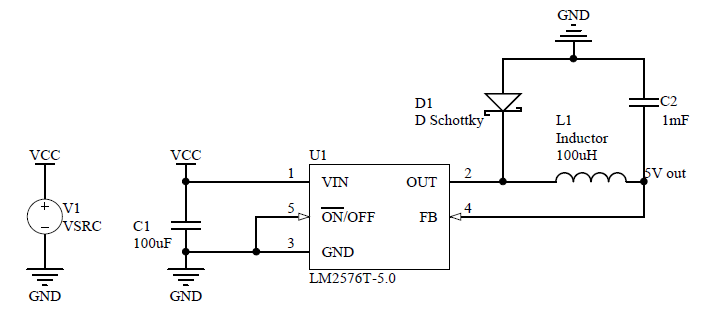
\includegraphics[scale=0.5]{fig/alim_5V.png}
\caption{Figure présentant les plans de l'alimentation 5V pour les périphériques}
\label{fig:alim5V}
\end{figure}

\begin{figure}[htbp]
\centering
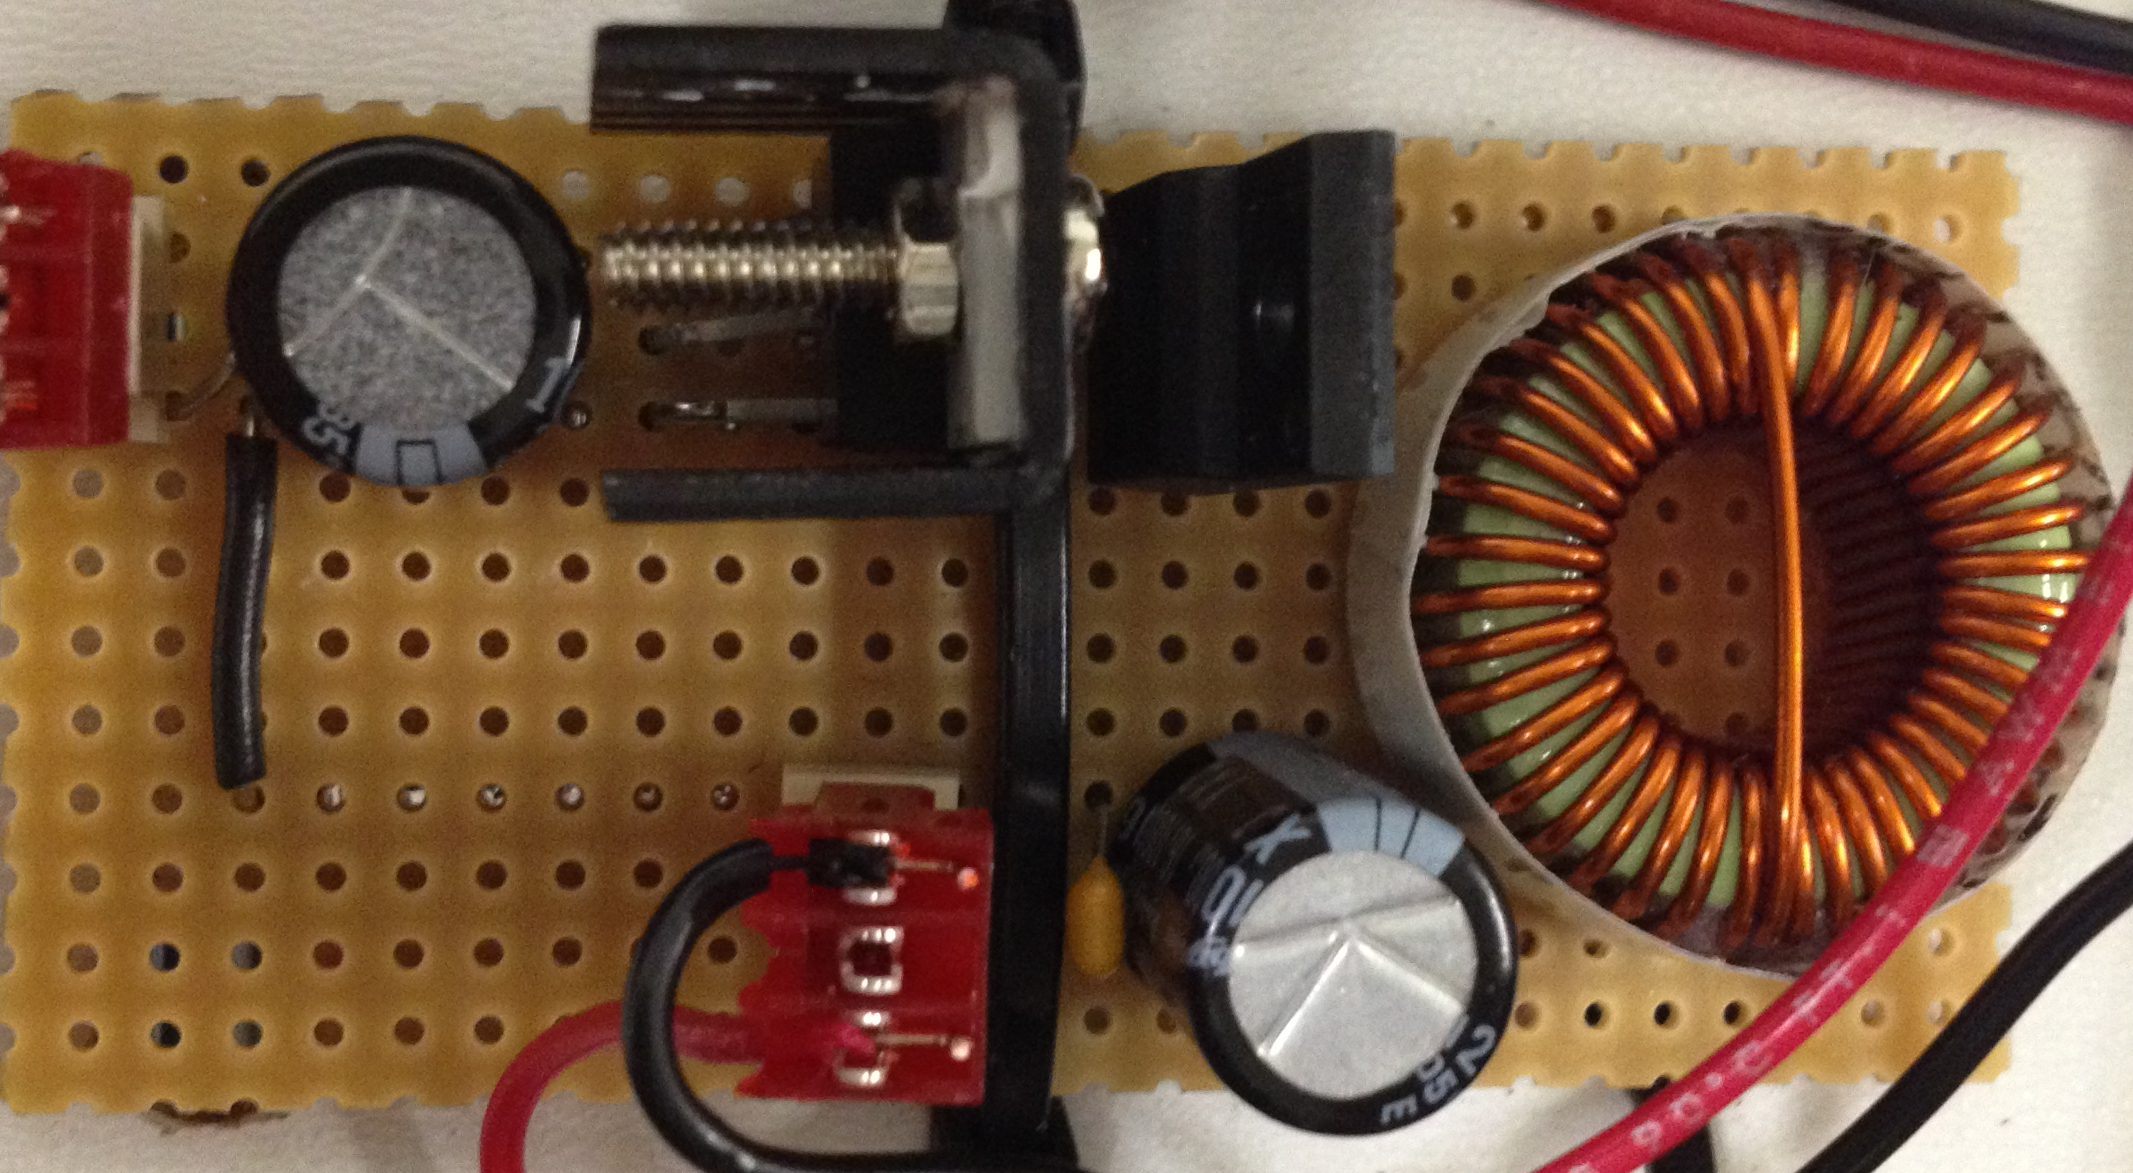
\includegraphics[scale=0.2]{fig/alim_5V_photo.png}
\caption{Figure présentant une photo de l'alimentation 5V pour les périphériques}
\label{fig:alim5Vphoto}
\end{figure}

\section{Alimentation du Mac mini}
L'alimentation du Mac mini a été réalisé au moyen d'un circuit de type Boost réglable, acheté déjà monté. Les plans ne sont pas disponibles, mais une photo du dispositif l'est à la figure \ref{fig:alim24Vphoto}.

\begin{figure}[htbp]
\centering
\includegraphics[scale=0.1]{fig/alim_24V_photo.png}
\caption{Figure présentant une photo de l'alimentation 24V pour les périphériques}
\label{fig:alim24Vphoto}
\end{figure}

\section{Asservissement des moteurs}
\subsection{Modélisation}
L'optimisation des paramètres de réglage a été réalisée grâce à l'utilisation d'un outil de CAO élaboré au moyen de Matlab-Simulink. La fonction de transfert des moteurs a été identifiée au moyen d'une réponse à l'échelon et de l'outil \textit{ident} de Matlab. L'ordre choisi de la fonction est élevé et présente une concordance de 94\% avec la réponse obtenue expérimentalement. L'outil \textit{pidtool} permet par la suite de configurer adéquatement le PIDF et d'obtenir la réponse souhaitée et les paramètres associés. Suivant ces paramètres, le PIDF présent dans le microcontrôleur est ajusté.
\paragraph{}L'usage de l'outil interactif permet d'optimiser la réponse et d'obtenir des paramètres de préréglages qui limitent le nombre d'itérations. La réponse obtenue logiciellement est présentée à la figure \ref{fig:as_1}
\begin{figure}[htbp]
\centering
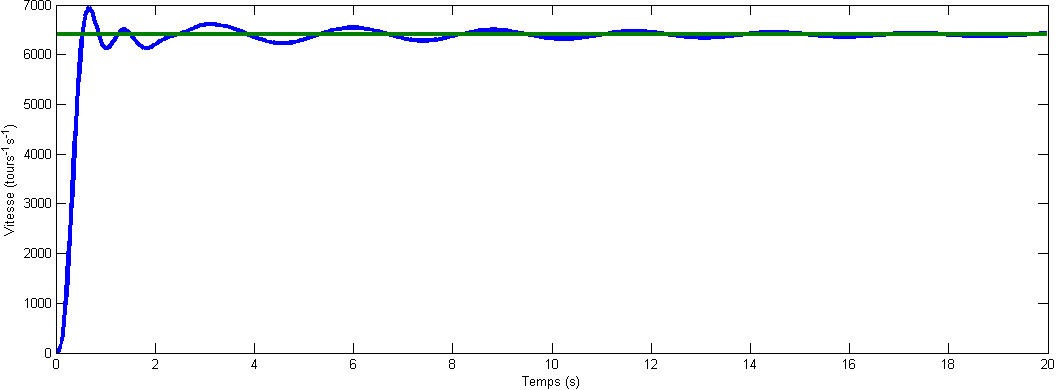
\includegraphics[scale=0.6]{fig/asservissement_1.png}
\caption{Figure présentant la réponse à un échelon de consigne de 6400$\left[tours^{-1}s^{-1}\right]$ du système régulé au moyen du régulateur optimisé dans simulink}
\label{fig:as_1}
\end{figure}
\subsection{Implantation pratique}
\label{s:ass_implantation_pratique}
La réponse à un échelon de consigne de 6400 ($tours^{-1} s^{-1}$) avec les paramètres de réglage réels est présentée à la figure \ref{fig:as_2}. À noter que les consignes en $tours^{-1} s^{-1}$ indique la vitesse en nombre de 1/6400 de tours de roue. Cette fraction de tour est due au fait que les interfaces d'encodeurs en quadratures captent 6400 transitions par tour complet de roue (voir la sous-section \ref{asservissement_mesures} pour plus de détails).
Le système a été implanté avec un asservissement en vitesse et sans asservissement de position. Les expériences pratiques réalisées montrent que l'évolution de la position est linéaire, et ce, sans asservissement. La figure \ref{fig:as_3} présente ce phénomène pour une consigne de 6400 ($tours^{-1} s^{-1}$) qui vise à amener le système à une position de 9100 $tours^{-1}$.
En utilisant les paramètres obtenus dans Matlab comme point de départ, les paramètres de réglages ont été modifiés de manière à obtenir des réponses remplissant les critères de stabilité, de vitesse et de dépassement souhaités. Afin d'améliorer la vitesse des déplacements, différents PID ont été ajustés selon différentes vitesses d'asservissement. On compte 3 de ces PID pour les déplacements unilatéraux et 1 déplacement réservé pour les mouvements reliés au dessin. La différence est que la vitesse de dessin est beaucoup plus basse que celle du déplacement usuel en vue de permettre une plus grande précision. Le moteur n'étant plus très linéaire à ces faibles vitesses (roulement et zone morte très limitants) et le système étant incapable de démarrer de lui même pour procéder à l'identification, le PID a donc été ajusté de manière manuelle, par itérations. Les PID sont fonctionnels et les systèmes stables, cependant, la décélération avant l'arrêt et le positionnement critique se font par l'entremise d'un palier de ralentissement à une vitesse intermédiaire avant freinage. Ces courbes de décélérations sont à mettre au point avant de pouvoir entamer le contrôle en dessin. Par ailleurs, les mouvements en diagonale ne sont pas encore parfaitement au point et requièrent quelques heures de travail additionnelles.
\begin{figure}[htbp]
\centering
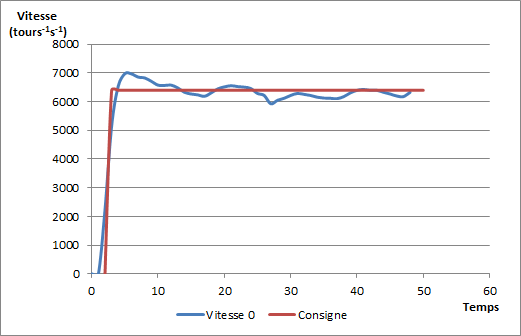
\includegraphics[scale=0.6]{fig/asservissement_3.png}
\caption{Figure présentant la réponse à un échelon de consigne de 6400$\left[tours^{-1}s^{-1}\right]$ du système régulé au moyen du régulateur réel et de la réponse en position associée}
\label{fig:as_2}
\end{figure}
\begin{figure}[htbp]
\centering
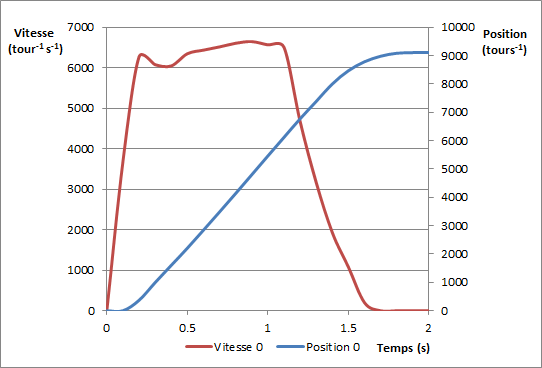
\includegraphics[scale=0.6]{fig/asservissement_2.png}
\caption{Figure présentant la réponse à un échelon de consigne de 6400$\left[tours^{-1}s^{-1}\right]$ du système régulé au moyen du régulateur réel et de la réponse en position associée}
\label{fig:as_3}
\end{figure}
\subsection{Implantation électronique}
\subsubsection{Les prises de mesures}
\label{asservissement_mesures}
Pour prendre des mesures de positions et de vitesses pour effectuer l'asservissement, nous utilisons deux QEI (Quadrature Encoder Interface) matériels qui sont sur le microcontrôleur. Ces deux interfaces prennent en entrée les sorties des encodeurs situés sur les moteurs et captent les transitions lors de la rotation des moteurs. Puisqu'il y a deux senseurs placés en quadrature sur chaque moteur, on peut détecter la direction de la rotation des moteurs. À prendre note qu'un signal transmis par un encodeur contient 64 transitions par tour complet de moteur et que le ratio de la rotation moteur:roue est 100:1. Un signal transmis par un encodeur contient alors 6400 transitions pour une rotation complète de roue. Pour les deux autres moteurs, nous avons réalisé deux interfaces d'encodeurs en quadratures logicielles à l'aide de deux broches d'entrées/sorties par interface, de courtes interruptions et d'une machine à états. Les interruptions sont lancées lorsqu'une transition est détectée sur l'une des broches. L'état des broches est alors lu et sauvegardé pour être traité par la machine à états. La machine à états utilisée est illustrée à la figure \ref{fig:cytron_machine_etats}. Les 0 et 1 indiqué dans les cercles identifient l'état logique des broches. Les -1 ou +1 tracés au dessus des transitions indiquent s'il faut incrémenter ou décrémenter la position de la roue en rotation.
\begin{figure}[htbp]
\centering
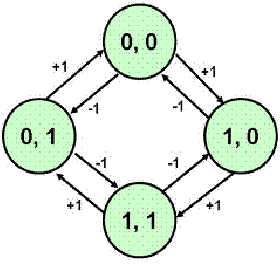
\includegraphics[scale=0.7]{fig/cytron_machine_etats.png}
\caption{Machine à états servant d'interface d'encodeur en quadrature (Cytron. Quadrature Encoder. \url{http://tutorial.cytron.com.my/2012/01/17/quadrature-encoder/}, consulté le 3 mars.)}
\label{fig:cytron_machine_etats}
\end{figure}
\subsubsection{PID}
Le PID utilisé pour l'asservissement est une courte fonction réalisée dans le microcontrôleur. Cette fonction se retrouve dans l'annexe \ref{s:fonction_PID}. À prendre note que l'argument "I" est l'intégrale de l'erreur et "dt" est la différence en temps entre chaque exécution de l'asservissement des moteurs. Cette fonction est exécutée individuellement pour chaque moteur. Des pointeurs transmis en argument indiquent l'emplacement en mémoire des valeurs de chaque moteur utilisées dans le PID. Ensuite, la fréquence d'exécution de la fonction est gardée constante à l'aide d'un timer dans le microcontrôleur qui déclenche une interruption à chaque période et lance l'exécution de l'asservissement.
\subsubsection{Ajustement de la vitesse selon la positon}
Comme indiqué précédemment, pour que le robot atteigne la consigne de position, la vitesse de la rotation des roues doit être ajustée selon la distance restante entre le robot et le point de destination. Cette ajustement est implanté par une simple multiplication d'un certain pourcentage avec la consigne de vitesse lorsque la distance restante à parcourir sera de "X" $tour^{-1}$. Le pourcentage utilisé présentement est hypothétique et sera ajusté lorsque les courbes de décélérations discutées dans la section \ref{s:ass_implantation_pratique} seront identifiées.

\section{Servomoteurs de la Webcam}
Pour contrôler les servomoteurs de la webcam, nous utilisons le contrôleur Micro Maestro de Pololu. Pour le programmer/configurer nous utilisons l'application "Maestro Control Center". Les servomoteurs et le Micro Maestro sont alimentés par l'alimentation 5V. De plus, les servomoteurs reprennent une position prédéterminée lorsque ceux-ci et le Micro Maestro sont alimentés et restent fixes pour permettre à la Webcam de rester immobile même lorsque le robot est en mouvement. Prochainement, un script sera implanté dans le Micro Maestro à l'aide du "Maestro Control Center" pour transmettre par USB une commande du Mac Mini au contrôleur un changement de position des servomoteurs. Cela a pour but de changer l'angle de la Webcam par rapport au sol. Ce changement est nécessaire pour détecter l'orientation du robot.

\section{Extraction des sudocubes}
\subsection{Composantes du système}
L'algorithme pour extraire les sudocubes est séparé en deux : une classe qui traite une photo afin d'extraire les informations d'un sudocube et un lecteur de chiffres. L'extracteur de sudocubes passe des images au lecteur de chiffres afin d'identifier le chiffre présent.

\begin{figure}[htbp]
\centering
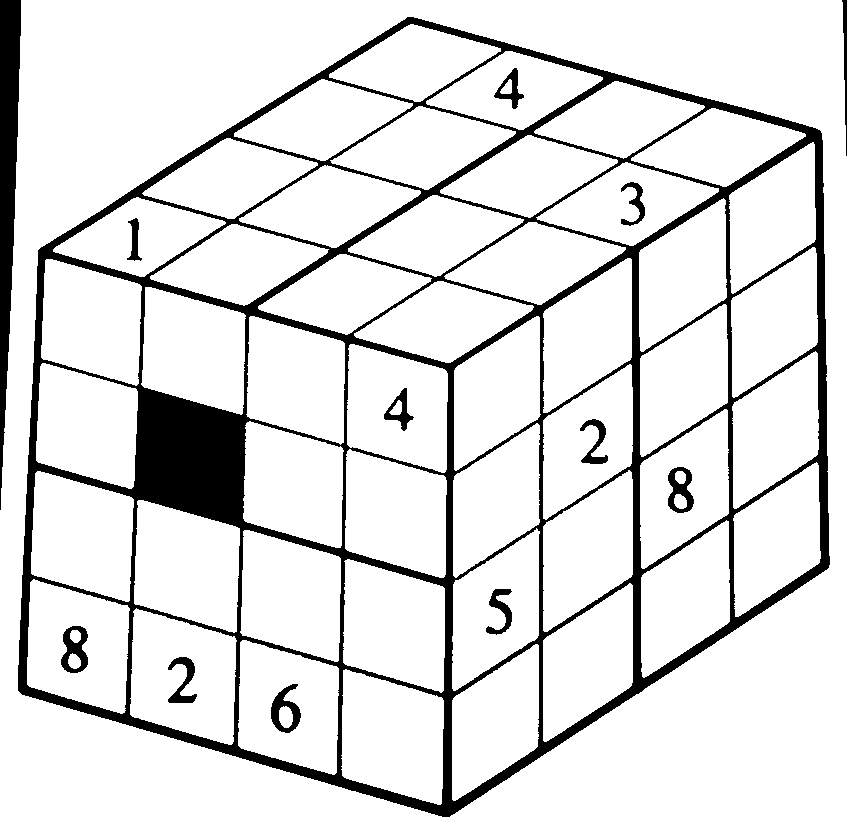
\includegraphics[scale=0.25]{fig/sudocubeThreshold.png}
\caption{Figure présentant un sudocube traité afin d'extraire les informations des cases}
\label{fig:sudoThresh}
\end{figure}

\begin{figure}[htbp]
\centering

\includegraphics[scale=0.9]{fig/chiffresLues.png}
\caption{Figure présentant un exemple d'images extraites des cases du sudocube et normalisées avant d'être passé au lecteur de chiffres}
\label{fig:chifLu}
\end{figure}

\subsection{Les solutions retenus/considérés}
Pour le lecteur de chiffres, deux solutions furent considérés : la librairie Tesseract et l'algorithme d'intelligence artificielle KNearest implanté dans la librairie OpenCV. Tesseract est une librairie qui permet de faire la lecture de caractères de plusieurs langues. Nous avons jugé que cette solution offre des fonctionnalités superflues en plus d'imposer une dépendance supplémentaire au projet. Puisque OpenCV est une dépendance obligatoire et que la méthode KNearest nous permet d'obtenir le même résultat qu'avec Tesseract nous avons choisit cette solution. 

\subsection{Les moyens utilisé pour configurer}
L'extracteur de sudocube fut configuré (valeur de threshold, coefficient de dilatation/d'érosion) à partir d'un lot de tests de 42 images(angles, distances sudocube/robot et luminosités variés). La configuration fut réalisé par essais/erreur pour trouver les paramètres optimal pour toutes les images.

Le lecteur de chiffres est entraîné avec 40 échantillons par chiffres. Aucune configuration supplémentaire nécessaire.

\section{Solveur de Sudocubes}
L'algorithme qui solve les sudocubes a été codé en C++. Malgré que l'utilisation de la programmation par contraintes (CSP) aurait été beaucoup plus simple à implanter et nous aurait fait économiser du temps, nous n'avions pas envisagé cette solution au départ. Au moment où nous avons entendu parler de ce type de programmation, nous avions presque terminé notre solution "maison". 

Le solveur utilise une structure de données afin de garder en mémoire le sudocube qui n'est en fait qu'un simple tableau à trois dimensions. Elle devient donc en même temps une interface pour la vision afin de stocker ses données obtenues lors de l'extraction du sudocube.

Les stratégies utilisées pour solutionner le sudocube sont les mêmes qui sont utilisées dans le monde des sudoku normaux, mais adaptées aux sudocubes. Plus spécifiquement, nous avons utilisé les stratégies (ici citées en anglais pour les retrouver plus facilement sur Internet):\newline

\begin{itemize}
\item Naked pairs
\item Hidden pairs/triples
\item Pointing pairs/triples
\item Box and line reduction
\end{itemize}

\paragraph{}Si ces stratégies ne suffisent pas à solutionner le sudocube, nous utilisons la technique de force brute. Nous pensons que c'est une solution acceptable puisque il sera plutôt rare que cette situation surviendra et même lorsque ça arrive, le temps d'exécution de l'algorithme reste sous un niveau acceptable.

L'algorithme est à présent fonctionnel. Il peut trouver une solution à des sudocubes ayant uniquement 4 chiffres au départ. Il satisfait donc les exigences du client étant donné que les sudokubes "test" présentés au laboratoires ont entre 9 et 14 chiffres. À l'heure actuelle, bien que nous sachions que l'algorithme fonctionne correctement, il resterait toutefois un refactoring à faire au niveau des classes afin d'améliorer la structure et la lisibilité du code, tout en respectant l'orienté-objet. De plus, il resterais quelques tests unitaitres et tests d'intégration à écrire afin de s'assurer de la robustesse du code.

\section{Recherche de chemin}
La fonctionnalité recherche de chemin n’en est encore qu’au stade prototype. Cette fonctionnalité n'a pas reçu beaucoup d'attention depuis le livrable 1. On pourrait donc se fier aux données énoncées dans ce livrable pour connare l'état de la recherche de chemin: "L'algorithme A* a été choisi, car il est très rapide et facile à implémenter". Nous savons que la solution développée dans le prototype est viable, mais il reste du travail à faire pour que ce soit fonctionnel. Il faudra entre autres ajouter une couche logicielle afin de réduire le nombre de points dans le chemin trouvé et ainsi réduire le nombre de rotations du robot.

\section{Communication microcontrôleur - Mac mini}

La communication entre le Mac mini a été réalisée avec un port série UART avec protocole RS-232 à travers le module ICDI du microcontrôleur LM3S9B92. Nous avons choisi ce protocole en raison de sa simplicité et de la facilité du déverminage par rapport au protocole USB plus complexe. Une interface de communication qui passe des commandes sous forme de caractères a été développée du côté microcontrôleur. Un terminal série écrit en Python et utilisant la librairie Pyserial a été développé du côté ordinateur. Ce terminal pour usage diagnostique est compatible avec Linux et Windows et permet de récolter des données utiles sous forme de fichiers CSV pour le développement et les tests d'asservissement et de décodage d'antenne. Le terminal final aura une forme légèrement différente afin de s'interfacer avec ROS.

\section{Décodage du signal Manchester - partie logicielle}

Le décodage logiciel du signal de l'antenne doit transformer les bits en encodage Manchester en bits traditionnels. La méthode choisie doit être robuste aux changements de taux de transmission de bits, car il est spécifié dans la description du projet que ce taux peut varier de plus ou moins 50 bits / seconde. Parmis les algorithmes permettant de détecter des signaux de taux de transmission inconnu, il en existe deux types principaux : 

\begin{enumerate}
\item{Les algorithmes basés sur l'échantillonnage}

On effectue une mesure du signal à un intervalle prédéfini plus petit que la période du signal mesuré. C'est le décompte des bits consécutifs à zéro et à un qui permet de décoder le signal.

\item{Les algorithmes basés sur les timings} 

On effectue une mesure du temps entre les transitions du signal de zéro à un et de un à zéro. C'est le temps entre les montées et descentes qui permet de décoder le signal.
\end{enumerate}

Puisque le LM3S9B92 possède des compteurs d'usage général qui implémentent une fonction de capture d'événement, nous avons choisi d'utiliser la méthode par timings. Pour l'instant, nous pouvons mesurer des temps entre transitions sur un signal interne au microcontrôleur généré par un PWM.


\section{Orientation du robot}

Pour la détermination d’angle et l’orientation du robot, le choix de la caméra embarquée  est très recommandé pour sa précision comparé à la kinect. En premier, on calibre la caméra, deux méthodes s’offrent à nous pour cette opération : l’application de l’algorithme de Zhang ou la calibration avec Opencv. Celle qui est retenue est la première, malgré sa complexité, elle est plus efficace. Ensuite, on procède à la détermination d’angle du robot par rapport à la ligne rouge déjà tracée sur la table, cette partie est réalisée grâce à un traitement d’image supportant la variation de luminosité, d’ombres… et des règles de trigonométrie. Finalement,  la détermination de l’orientation du robot (N, S, E, O) est effectuée par la détection des coins de la table. L’algorithme de cette opération est assez simple, si la caméra détecte : Orange avant bleu (orienté vers le Nord), bleu avant orange (orienté vers le Sud), les deux coins bleu (orienté vers le Ouest), les deux coins orange (orienté vers le Est). Les deux dernières parties sont commencées mais ne sont pas encore complétées à ce jour.

\section{Vision par Kinect}
Pour aider au déplacement du robot, la Kinect à été utilisée pour détecter la position des obstacles, la position du robot lui-même ainsi que sa position angulaire par rapport au point (0.0) de notre représentation cartésienne de la table. Toutefois, comme la Kinect est située à l'extérieur de la table de jeu, il a fallu effectuer une translation et une rotation des données obtenues pour positionner avec exactitude les objets. Les 3 sections qui suivent expliquent en détail les différentes parties de l'algorithme de vision de la Kinect.

\subsection{Transformation des distances}
En premier lieu, il est important de clarifier quelles distances il est possible d'obtenir à l'aide de la Kinect. Le «Framework» OpenNI est capable de retourner 2 types de distances pour chacun des points dans l'image infrarouge obtenue de la Kinect. Le premier type de distances retourné est la longueur en mètre entre l'objectif et un point quelquonque sur l'image. Le second type est dérivé du premier et correspond aux composantes X, Y et Z du vecteur de longueur entre l'objectif et la cible. Pour aider à la compréhension, les deux types de distances peuvent être représenté par les ligne verte sur l'image \ref{fig:kinect_distance}. Toutefois, comme l'origine de notre représentation cartésienne de la table est situé sur le coin inférieur droit de la table et que la Kinect n'est pas situé à cet endroit, il est nécessaire d'obtenir la distance X et Y (lignes bleues sur l'image \ref{fig:kinect_distance}) entre l'origine et le point ciblé sur l'image obtenue de la Kinect. Pour y arriver, il suffit d'obtenir la position X et Y (lignes rouges sur l'image \ref{fig:kinect_distance}) de la lentille infrarouge de la Kinect ainsi que l'angle de la Kinect avec l'axe X de la table. Avec ces valeurs, dans notre cas 14cm, -56cm et $23.5^o$, nous avons mis en oeuvre un logiciel qui permet la transformation des distances de la Kinect vers les composantes X et Y recherchée à l'aide de règles de trigonométrie simples. Cet algorithme permet d'obtenir avec une précision de plus ou moins 1cm pour n'importe quel point situé sur l'image obtenue avec la Kinect. 

\begin{figure}[htbp]
\centering
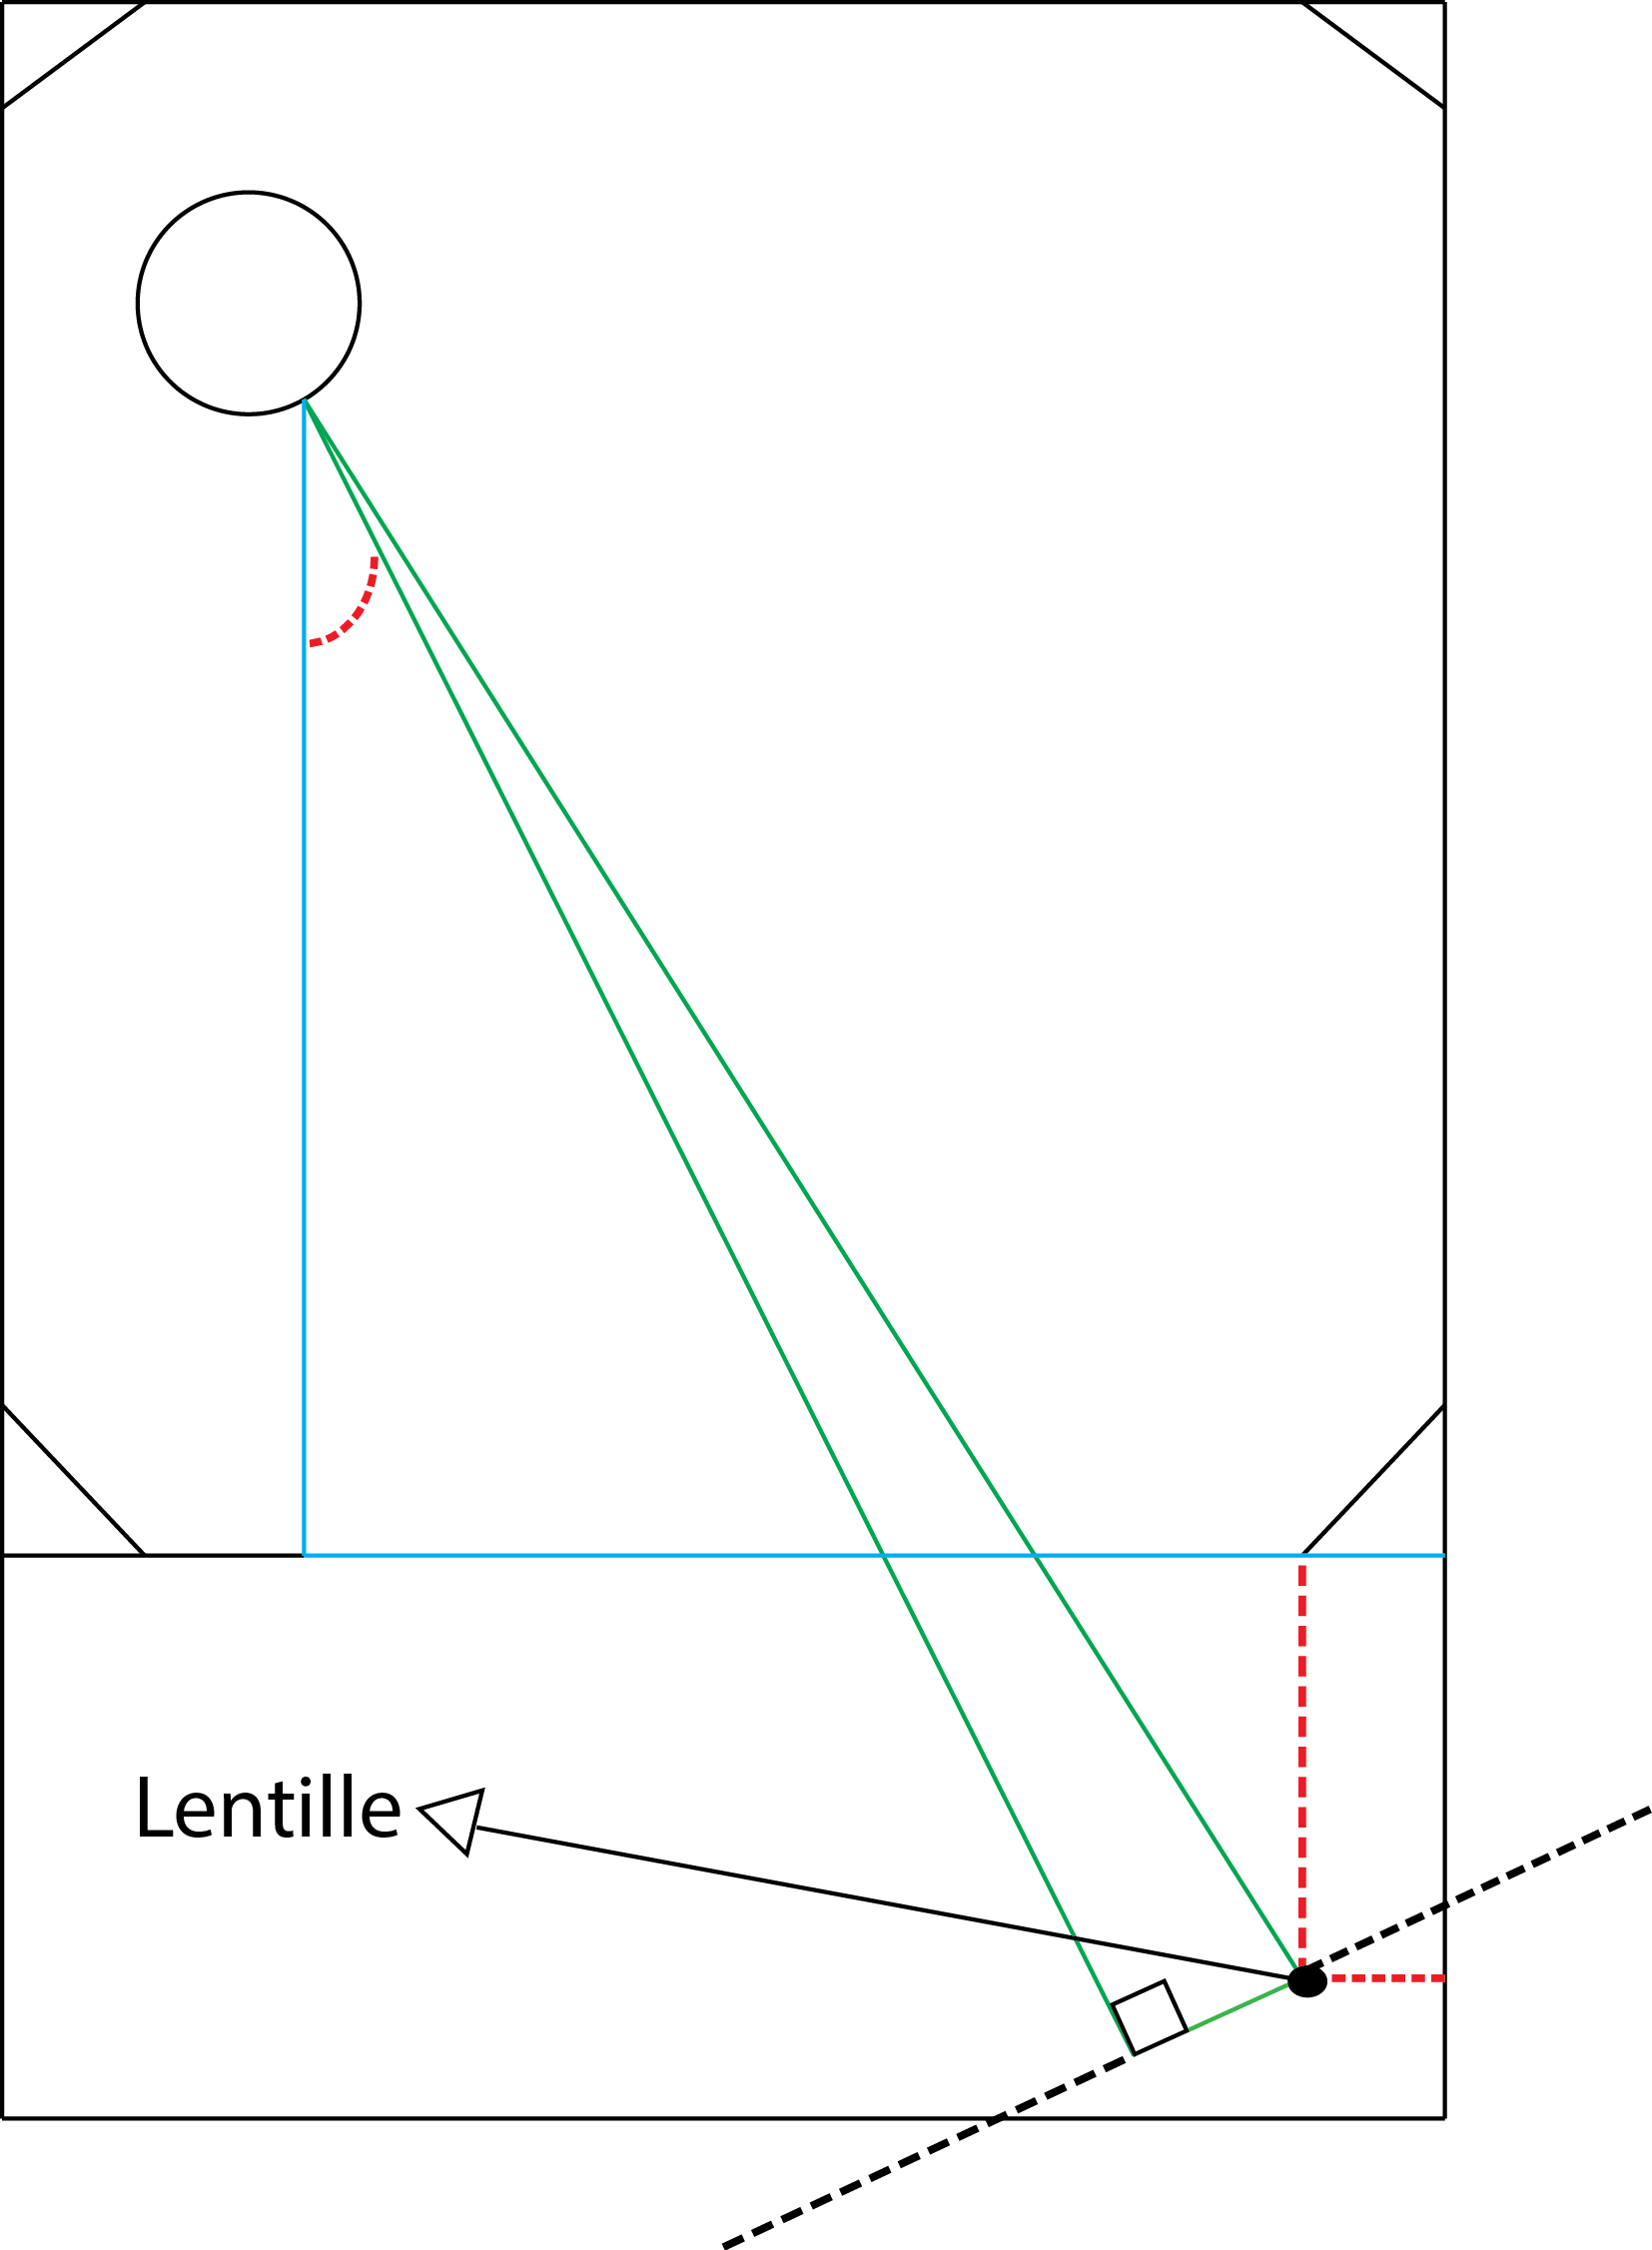
\includegraphics[scale=0.5]{fig/kinect_distance.png}
\caption{Schéma représentant la table et les différentes mesures obtenues avec la Kinect pour un point quelquonque}
\label{fig:kinect_distance}
\end{figure}

\subsection{Détection des obstacles}
Maintenant que nous pouvons obtenir n'importe quelle distance entre l'origine et un point quelquonque sur l'image, nous avons créé l'algorithme de recherche d'obstacles. Sachant que les obstacles sont situés dans une zone précise sur la table et que ceux-ci font 40cm de hauteur, il suffit de rechercher tout objet de cette hauteur et situé dans la zone prédefinie. Comme la Kinect est capable de retourner la hauteur de chacun des points sur l'image infrarouge, il a été facile de trouver les obstacles de cette manière. De plus, à l'aide de simples calculs de statistiques, notre programme est capable de trouver les obstacles qui sont presque enlignés ou bien les obstacles avec obstructions devant eux. Comme cet algorithme dépend entièrement de l'algorithme précédent, les positions obtenues pour chacun des obstacles possèdent la même incertitude de 1 cm sur chaque mesure de distance effectuée.

\subsection{Détection du robot}

\section{Communication entre le Mac mini et la station de base}
\subsection{Composantes du système}
Avant de pouvoir communiquer avec le robot nous récupérons l’adresse ip du robot grâce à un script bash exécuté lors du démarrage de celui-ci. Le script récupère l’adresse ip et l’envoie sur le site pastebin.com.

Ensuite, nous utilisons ROS pour gérer les communications entre le mac-mini et la station de base. Actuellement, nous avons testé l’envoie d’un message, à partir de la station de base, au Mac mini pour démarrer la séquence du robot.

Voir la section développement logiciel pour avoir plus d’information sur l’organisation des composantes du système. 

\subsection{Les solutions retenus/considérés}
Nous avons considérés deux solutions : POCO une librairie C++ et ROS un environnement de développement pour robot.

POCO permet d’envoyer des chaines de caractères par TCP/IP. L’envoie de commandes avec POCO consiste en ces étapes : concaténer le nom d’une commande (choisit au préalable) et ses arguments dans une chaine de caractères. Puis, envoyer, à l’aide de la librairie la chaine de caractères. Il faut extraire la commande et ses paramètres lors de la réception d’un message.

ROS fait exactement la même chose que POCO en arrière-plan, mais  il y a une couche logiciel qui nous donne des avantages supplémentaires. Pour envoyer des message entres deux applications ROS iI suffit de déclarer, pour chaque type de message, des variables et leur type dans un fichier texte. Puis, lors de la compilation du projet ROS génère des struct en C pour chaques message. Ensuite, on utilise l’api de ROS pour définir le contenu des messages et envoyer les messages.

La courbe d’apprentissage est nettement plus prononcé avec ROS. Cependant, avec celui-ci les messages sont hâchés avec une somme MD5 et lorsqu’un message est reçu par une node (une application ROS) le contenu est vérifié avec la somme MD5. Nous garantissant ainsi que le message s’est bien transmit.

De plus, il est possible d’enregistrer tous les messages qui sont envoyés par ROS depuis le démarrage de la séquence, de les consulter séquentiellement dans le temps grâce à une interface graphique et de les réexécuter afin de reproduire la même séquence. C’est un outil de déverminage qui sera utile lors du développement de l’agent intelligent et que l’on ne possède pas avec POCO.

ROS a été retenu pour ses nombreux avantages. 
